\documentclass{beamer}
\usepackage[utf8]{inputenc}
\usepackage{polski}
% \usepackage[polish]{babel}
\usepackage[T1]{fontenc}
\usepackage{tikz}
\usepackage{tikzducks}
% \usetikzlibrary{decorations.pathmorphing}
\usepackage{multimedia}
\usepackage{graphicx}
\usepackage[justification=centering]{caption}
\usepackage{textcomp}
\usepackage{appendixnumberbeamer}
\usepackage{qrcode}
% \usepackage[natbib, language=polish, sorting=none]{biblatex}
% \addbibresource{lio.bib}
\usepackage{hyperref}
%\usepackage[width=\textwidth]{animate}
%\usepackage{chemformula}
\usepackage{sidecap}
\usepackage{multirow}
\usepackage{rotating}
\usepackage{anyfontsize} % change font size for semposiwko

\usepackage{listings}
\lstset{
basicstyle=\small\ttfamily,
columns=flexible,
breaklines=true
}

\usepackage{emoji}
\usepackage{subcaption}


\usepackage[natbib, language=polish, sorting=none]{biblatex}
\addbibresource{lio.bib}
\renewcommand*{\bibfont}{\scriptsize}

\usetheme{Szeged}
\usecolortheme{whale}
\setbeamercolor{palette primary}{bg=violet!80!black,fg=white}
\setbeamercolor{palette secondary}{bg=violet!60!black,fg=white}
\setbeamercolor{palette tertiary}{bg=violet!40!black,fg=white}
\setbeamercolor{palette quaternary}{bg=violet!20!black,fg=white}
\setbeamercolor{structure}{fg=violet!60!black}
\setbeamertemplate{caption}{\insertcaption}
% \setbeamertemplate{headline}{
%   \begin{beamercolorbox}[wd=.9\paperwidth]{headline}
%     \vspace{1.5ex}
%     \insertsectionnavigationhorizontal
%     \vspace{1.5ex}
%   \end{beamercolorbox}
% }

\linespread{0.6}

% \setbeamertemplate{background}%
% {%
%     \begin{tikzpicture}[remember picture,overlay]{\node[yshift=1.5cm,xshift=-2cm,opacity=0.1] at (current page.south east)
%       {
%       \includegraphics[scale=0.4, angle=20]{ptaki.pdf}
%       }
%       ;
%     \node[yshift=1.0cm,xshift=0.6cm] (logopos) at (current page.south west) {{\begin{tikzpicture}\shuffleducks\duck[signpost=\insertframenumber, \randomhead,scale=.4]\end{tikzpicture}}};
%     \pgfmathsetmacro{\progress}{360*(\insertframenumber)/(\inserttotalframenumber)};
%     \draw[line width=0.2*3pt] ([xshift=0.55cm] logopos)  arc[radius=0.55cm, start angle=0, end angle=\progress];
%     \fill ([shift={(\progress:0.55cm)}] logopos) circle(1pt);

%     }
%         \end{tikzpicture}
    
% }

\newcommand{\SeMPowisko}{%
\large S\normalsize%
\kern-.3em \lower.2ex\hbox{e}%
\lower.2ex\hbox{\large M\normalsize}%
\kern-.1em \raise.1ex\hbox{\large P\normalsize}%
\kern-.3em \lower.2ex\hbox{o}%
\kern-.2em \raise.2ex\hbox{w}%
\lower.2ex\hbox{i}%
s%
\raise.2ex\hbox{k}%
\kern-.3em \lower.2ex\hbox{o}%
}

\newcommand\Tikz{Ti\emph{k}Z}
\definecolor{neworange}{RGB}{255,140,0}


\title{\Tikz}
\subtitle{od zera do elipsy}
\author[M. Winiarski]{Mateusz (czarny) Winiarski \& ChatGPT}
\institute[KMPS UJ]{KMPS UJ, WFAIS}
\date[dzisiaj]{dzisiaj}

\begin{document}

\frame{\titlepage}

\section{Co to \Tikz}

\begin{frame}{Co to \Tikz}
    \begin{itemize}[<+->]
        \item \Tikz{} ist \emph{keine} Zeichenprogramm
        \begin{itemize}[<+->]
            \item \Tikz{} to \emph{nie} program do rysowania
        \end{itemize}
        \item więc \Tikz{} to biblioteka (mniej więcej) w \LaTeX{}u do robienia obrazków (samemu!)
    \end{itemize}
\end{frame}

\begin{frame}{Skąd się tego nauczyć?}
tak jak zawsze:

szukamy w ulubionej wyszukiwarce internetowej \texttt{ctan tikz}...
\onslide<2->\begin{figure}
    \centering
    
\includegraphics[width=\textwidth]{tikz/Zrzut ekranu 2024-11-29 120331.png}
\end{figure}
\only<3->{klikamy w pierwszy link...\footnote{to nie jest ten link. to nie jest również moja ulubiona wyszukiwarka}}
\end{frame}

\begin{frame}{...}
    ...otwieramy dokumentację...
    \begin{figure}
        \centering
        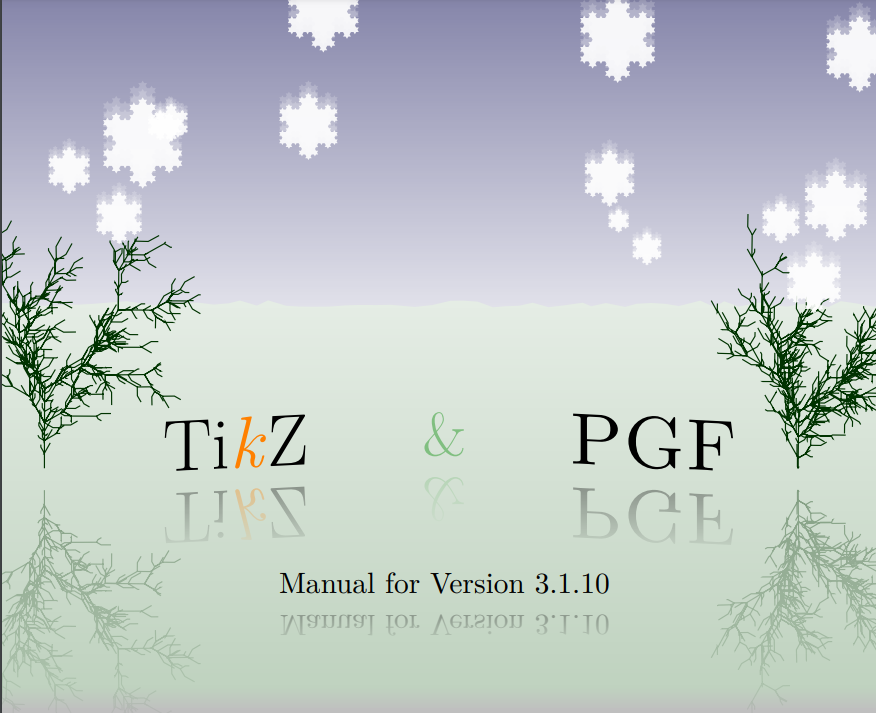
\includegraphics[width=0.6\textwidth]{tikz/Zrzut ekranu 2024-11-29 125324.png}
        \caption{ładny rysunek}
    \end{figure}
\end{frame}

\begin{frame}{...}
    ...płaczemy...
    \begin{figure}
        \centering
        
\includegraphics[width=0.9\textwidth]{tikz/Zrzut ekranu 2024-11-29 130423.png}
        \caption{\emoji{loudly-crying-face}}
    \end{figure}
\end{frame}

\begin{frame}{...}
    ...szukamy lepszego pdfa
    \begin{figure}
        \centering
        
\includegraphics[width=0.8\textwidth]{tikz/Zrzut ekranu 2024-11-29 132732.png}
        \caption{Z tego \texttt{pdf}a się uczyłem\footnote{tydzień temu}, i z niego będę uczył was}
    \end{figure}
\end{frame}

\begin{frame}{Ale ja nie rozumiem...}
    \emph{Internet is your friend}
    
    w szczególności:
    \begin{itemize}
        \item ChatGPT
        \item \TeX{} Stack Exchange
    \end{itemize}
\end{frame}

\begin{frame}[fragile]{Jak zacząć?}
    w preambule:
    
    \begin{verbatim}
    \usepackage{tikz}
    \end{verbatim}
    
    w dokumencie:
    
    \begin{verbatim}
    \begin{tikzpicture}
        % wpisz tu swój rysunek...
    \end{tikzpicture}
    \end{verbatim}\pause
    
    warto rozważyć:
    \begin{verbatim}
    \documentclass[margin=5mm]{standalone}
    \end{verbatim}
\end{frame}

\section{Kreski}

\begin{frame}[fragile]{\textrm{\emph{Hello, world!}}}{}
    \begin{verbatim}
\begin{tikzpicture}
    \draw (0,0) -- (1,2);
\end{tikzpicture}
    \end{verbatim}
    
czytaj jako:

\emph{\Tikz{}ie, narysuj mi kreskę od $(0,0)$ do $(1,2)$;}

wynik:
    
\begin{tikzpicture}
\draw (0,0) --(1,2);
\end{tikzpicture}
\end{frame}

\begin{frame}[fragile]{Ale fajne, chcę więcej}
    \begin{verbatim}
\begin{tikzpicture}
    \draw[thick] (0,0) -- (1,2) -- (2,2) -- (2,0);
\end{tikzpicture}
    \end{verbatim}
    
czytaj jako:

\emph{\Tikz{}ie, narysuj mi \textbf{tłustą} kreskę od $(0,0)$ do $(1,2)$, potem do $(2,2)$, potem do $(2,0)$;}

wynik:
    
\begin{tikzpicture}
\draw[thick] (0,0) -- (1,2) -- (2,2) -- (2,0);
\end{tikzpicture}
\end{frame}

\begin{frame}[fragile]{Wincyj!}
    \begin{verbatim}
\begin{tikzpicture}
    \draw[thick, red, fill=cyan]
        (0,0) -- (1,2) -- (2,2) -- (2,0) -- cycle;
\end{tikzpicture}
    \end{verbatim}
    
czytaj jako:

\emph{\Tikz{}ie, narysuj mi {\color{red} \textbf{czerwoną tłustą}} kreskę od $(0,0)$ do $(1,2)$, potem do $(2,2)$, potem do $(2,0)$, potem wróć, a wypełnij {\color{cyan} cyjanowo};}

wynik:
    
\begin{tikzpicture}
    \draw[thick, red, fill=cyan]
        (0,0) -- (1,2) -- (2,2) -- (2,0) -- cycle;
\end{tikzpicture}
\end{frame}

\begin{frame}[fragile]{Wincyj!!!}
    \begin{verbatim}
\begin{tikzpicture}
    \draw[thick, green, fill=yellow]
        (0,0) -- ++(1,2) -- ++(1,0) -- ++(0,-2) -- cycle;
\end{tikzpicture}
    \end{verbatim}
    
czytaj jako:

\emph{\Tikz{}ie, narysuj mi {\color{green} \textbf{zieloną tłustą}} kreskę od $(0,0)$, idź o wektor $(1,2)$, potem o wiktor $(1,0)$, potem o wektor $(0,-2)$, potem wróć, a wypełnij {\color{yellow} rzułto};}

wynik:
    
\begin{tikzpicture}
    \draw[thick, green, fill=yellow]
        (0,0) -- ++(1,2) -- ++(1,0) -- ++(0,-2) -- cycle;
\end{tikzpicture}
\end{frame}

\begin{frame}[fragile]{To widzisz już ogólną tendencję:}{}
    \begin{verbatim}
    \draw[opcje...] (punkt1) figura (punkt2);
    \end{verbatim}
czytaj jako:

\emph{\Tikz{}ie, narysuj mi figurę od $punkt1$ do $punkt2$ z podanymi opcjami;}


\end{frame}

\begin{frame}[fragile]{Czy mogę dać więcej na jednym rysunku?}{}
Tak, i to dokładnie w taki sposób w jaki się domyślasz:

    \begin{lstlisting}
\begin{tikzpicture}
    \draw[thick, red, fill=cyan] (0,0) -- (1,2) -- (2,2) -- (2,0) -- cycle;
    \draw[thick, green, fill=yellow]
        (1,1) -- ++(1,2) -- ++(1,0) -- ++(0,-2) -- cycle;
\end{tikzpicture}
    \end{lstlisting}
    
\begin{tikzpicture}
    \draw[thick, red, fill=cyan] (0,0) -- (1,2) -- (2,2) -- (2,0) -- cycle;
    \draw[thick, green, fill=yellow]
        (1,1) -- ++(1,2) -- ++(1,0) -- ++(0,-2) -- cycle;
\end{tikzpicture}

\end{frame}

\section{Kolorki}

\begin{frame}[fragile]{Kolorki}

Wiemy już, że kolory możemy definiować tak:

\verb|orange| \textcolor{orange}{pomarańczowy}

oraz tak:

\verb|\definecolor{neworange}{RGB}{255,140,0}| \textcolor{neworange}{pomarańczowy}\pause

ale jeszcze nie wiemy, że możemy tak:

\verb|orange!80!black| \textcolor{orange!80!black}{pomarańczowy}
    
\end{frame}

\begin{frame}[fragile]{Siatki}{}
\begin{verbatim}
\begin{tikzpicture}
    \draw[gray!50, step=0.2cm] (-5,0) grid (5,5);
    \draw[gray, step=1cm] (-5,0) grid (5,5);
    \draw[black, step=5cm] (-5,0) grid (5,5);
\end{tikzpicture}
\end{verbatim}
\begin{tikzpicture}
\draw[gray!50, step=0.2cm] (-5,0) grid (5,5);
\draw[gray, step=1cm] (-5,0) grid (5,5);
\draw[black, step=5cm] (-5,0) grid (5,5);
\end{tikzpicture}
\end{frame}

\section{Węzły i kolanka}

\begin{frame}[fragile]{Węzły}{}
\begin{columns}
\column{1\textwidth}
\begin{verbatim}
\begin{tikzpicture}
    \draw [thick, <->] (0,2) -- (0,0) -- (2,0);
    \node at (1,1) {andrzej};
\end{tikzpicture}
\end{verbatim}

% \column{0.5\textwidth}
\begin{tikzpicture}
\draw [thick, <->] (0,2) -- (0,0) -- (2,0);
\node at (1,1) {andrzej};
\end{tikzpicture}

\end{columns}
\end{frame}


\begin{frame}[fragile]{Kolanka}{}
\begin{columns}
\column{1\textwidth}
\begin{verbatim}
\begin{tikzpicture}
    \draw [thick, <->] (0,2) -- (0,0) -- (2,0);
    \draw[fill] (1,1) circle [radius=0.025];
    \node [below] at (1,1) {below};
    \node [above] at (1,1) {above};
    \node [left] at (1,1) {left};
    \node [right] at (1,1) {right};
\end{tikzpicture}
\end{verbatim}

% \column{0.5\textwidth}
\begin{tikzpicture}
\draw [thick, <->] (0,2) -- (0,0) -- (2,0);
\draw[fill] (1,1) circle [radius=0.025];
\node [below] at (1,1) {below};
\node [above] at (1,1) {above};
\node [left] at (1,1) {left};
\node [right] at (1,1) {right};
\end{tikzpicture}\hspace{2cm}\begin{tikzpicture}
\draw [thick, <->] (0,2) -- (0,0) -- (2,0);
\draw[fill] (1,1) circle [radius=0.025];
\node [below left] at (1,1) {below left};
\node [above left] at (1,1) {above left};
\node [below right] at (1,1) {below right};
\node [above right] at (1,1) {above right};
\end{tikzpicture}

\end{columns}
\end{frame}

\begin{frame}[fragile]{Wincyj kolanek}
\begin{lstlisting}
\begin{tikzpicture}
\draw[thick, green, fill=yellow](0,0) node [below left] {A} -- ++(1,2) node [above left] {B} -- ++(1,0) node [above right] {C} -- ++(0,-2) node [below right] {D} -- cycle;
\end{tikzpicture}
\end{lstlisting}


\begin{tikzpicture}
\draw[thick, green, fill=yellow](0,0) node [below left] {A} -- ++(1,2) node [above left] {B} -- ++(1,0) node [above right] {C} -- ++(0,-2) node [below right] {D} -- cycle;
\end{tikzpicture}
    
\end{frame}

\begin{frame}[fragile]{Koordynaty}{}
\begin{lstlisting}
\begin{tikzpicture}
    \coordinate (A) at (0,0);
    \coordinate (B) at (1,2);
    \draw[thick, green, fill=yellow] (A) node [below left] {A} -- (B) node [above left] {B} -- ++(1,0) node [above right] {C} -- ++(0,-2) node [below right] {D} -- cycle;
\end{tikzpicture}
\end{lstlisting}

\begin{tikzpicture}
\coordinate (A) at (0,0);
\coordinate (B) at (1,2);
\draw[thick, green, fill=yellow] (A) node [below left] {A} -- (B) node [above left] {B} -- ++(1,0) node [above right] {C} -- ++(0,-2) node [below right] {D} -- cycle;
\end{tikzpicture}
\end{frame}

\section{Już nie kreski}

\begin{frame}[fragile]{Prostokąt}{}
\begin{columns}
\column{0.5\textwidth}
\begin{lstlisting}
\begin{tikzpicture}
\coordinate (A) at (0,0);
\coordinate (B) at (4,2);
    \draw[thick, green, fill=yellow] (A) rectangle (B) ;
\end{tikzpicture}
\end{lstlisting}
\begin{tikzpicture}
\coordinate (A) at (0,0);
\coordinate (B) at (4,2);
    \draw[thick, green, fill=yellow] (A) rectangle (B) ;
\end{tikzpicture}
\column{0.5\textwidth}
\begin{lstlisting}
\begin{tikzpicture}
\coordinate (A) at (0,0);
\coordinate (B) at (4,2);
    \draw[thick, green, fill=yellow, rounded corners = 1 cm] (A) rectangle (B) ;
\end{tikzpicture}
\end{lstlisting}
\begin{tikzpicture}
\coordinate (A) at (0,0);
\coordinate (B) at (4,2);
    \draw[thick, green, fill=yellow, rounded corners = 1 cm] (A) rectangle (B) ;
\end{tikzpicture}
\end{columns}
\end{frame}

\begin{frame}[fragile]{Kółko i elipsa}{}
\begin{columns}

\column{0.5\textwidth}
\begin{lstlisting}
\begin{tikzpicture}
\coordinate (A) at (0,0);
    \draw[thick, green, fill=yellow] (A) circle(1 cm) ;
\end{tikzpicture}
\end{lstlisting}
\begin{tikzpicture}
\coordinate (A) at (0,0);
    \draw[thick, green, fill=yellow] (A) circle(1 cm) ;
\end{tikzpicture}
    
\column{0.5\textwidth}
\begin{lstlisting}
\begin{tikzpicture}
\coordinate (A) at (0,0);
    \draw[thick, green, fill=yellow] (A) ellipse[x radius={sqrt(2)}, y radius={sin(90)}] ;
\end{tikzpicture}
\end{lstlisting}
\begin{tikzpicture}
\coordinate (A) at (0,0);
    \draw[thick, green, fill=yellow] (A) ellipse[x radius={sqrt(2)}, y radius={sin(90)} ] ;
\end{tikzpicture}

\end{columns}
\end{frame}



\begin{frame}[fragile]{Łuki}{}
\begin{columns}
\column{0.5\textwidth}
\begin{lstlisting}
\begin{tikzpicture}
    \draw[->, dashed, fill=orange, very thick] (3,0) arc [start angle=0, end angle=90, radius=3 cm];
\end{tikzpicture}
\end{lstlisting}
\begin{tikzpicture}
    \draw[->, dashed, fill=orange, very thick] (3,0) arc [start angle=0, end angle=90, radius=3 cm];
\end{tikzpicture}

\column{0.5\textwidth}
\begin{lstlisting}
\begin{tikzpicture}
    \draw[<->, thick, orange] (3,0) arc [start angle=180, end angle=390, radius=2 cm] -- (5,0) -- cycle;
\end{tikzpicture}
\end{lstlisting}
\begin{tikzpicture}
    \draw[<->, thick, orange] (3,0) arc [start angle=180, end angle=390, radius=2 cm] -- (5,0) -- cycle;
\end{tikzpicture}
\end{columns}

    
\end{frame}

\begin{frame}[fragile]{Krzywe B\'eziera}{}
    \begin{figure}
        \centering
        \begin{subfigure}{0.45\textwidth}
        \includegraphics[width=0.9\textwidth]{tikz/Bézier_2_big.svg.png}
        \end{subfigure}
        \begin{subfigure}{0.45\textwidth}
        \includegraphics[width=0.9\textwidth]{tikz/Bézier_3_big.svg.png}
        \end{subfigure}
        \caption{Rysunek z \url{https://en.wikipedia.org/wiki/Bezier_curve}}
        % \label{fig:my_label}
    \end{figure}\pause
    \begin{columns}
    \column{0.3\textwidth}
    \begin{tikzpicture}
    \draw[thick,orange] (0,0) .. controls (-0.5,1) .. (2,0);
    \draw[thick,red] (0,0) .. controls (-0.5,1) and (1,1) .. (2,0);
    \node at (-0.5,1) {$\bullet$};
    \node at (1,1) {$\bullet$};
    \end{tikzpicture}
    \column{0.7\textwidth}
    \begin{lstlisting}
\begin{tikzpicture}
    \draw[thick,orange] (0,0) .. controls (-0.5,1) .. (2,0);
    \draw[thick,red] (0,0) .. controls (-0.5,1) and (1,1) .. (2,0);
    \node at (-0.5,1) {$\bullet$};
    \node at (1,1) {$\bullet$};
\end{tikzpicture}
    \end{lstlisting}
    \end{columns}
\end{frame}

\section{Ćwiczenia}

\begin{frame}{Ćwiczenia I}{}
\begin{columns}
\column{0.5\textwidth}
\begin{figure}
    \begin{tikzpicture}
    % Współrzędne środków
    \coordinate (A) at (0, 0);
    \coordinate (B) at (1, 0);
    \coordinate (C) at (2, {4 * sqrt(3)/2 - 3});
    
    % Kształty
    \draw[very thick, red, fill=green!50!black] (A) circle(1cm); % Koło
    \draw[thick, dashed, blue] (B) -- ++(-1, {-sqrt(3)}) -- ++(2, 0) -- cycle; % Trójkąt równoboczny
    \draw[thin, red] (C) rectangle ++(2, 2); % Kwadrat
\end{tikzpicture}
\caption{Zadanie 1}
\end{figure}
\column{0.5\textwidth}
\begin{figure}
\begin{tikzpicture}
    % Wierzchołki
    \coordinate (A) at (0, 0);
    \coordinate (B) at (4, 0);
    \coordinate (C) at (4, 2);
    \coordinate (D) at (0, 2);
    
    % Prostokąt
    \draw[thick] (A) -- (B) -- (C) -- (D) -- cycle;
    
    % Przekątne
    \draw[thick, dashed] (A) -- (C);
    \draw[thick, dashed] (B) -- (D);
    
    % Oznaczenia wierzchołków
    \node[below left] at (A) {A};
    \node[below right] at (B) {B};
    \node[above right] at (C) {C};
    \node[above left] at (D) {D};
\end{tikzpicture}
\caption{Zadanie 2. Wskazówka: użyj koordynatów}
\end{figure}
\end{columns}
\end{frame}

\begin{frame}{Ćwiczenia II}
\begin{columns}
\column{0.5\textwidth}
\begin{figure}
    \begin{tikzpicture}
    % Parametry
    \def\F{3}      % Długość wektora siły F
    \def\angle{30} % Kąt siły F (w stopniach)
    \def\m{1.5}    % Wysokość prostokąta reprezentującego ciało

    % Ciało
    \draw[thick] (0,0) rectangle (2,\m) node[midway] {$m$};

    % Siły
    % Siła ciężkości
    \draw[->, thick, blue] (1, 0) -- ++(0, -2) node[midway, left] {$\vec{F}_g$};
    
    % Siła normalna
    \draw[->, thick, green!70!black] (1, \m) -- ++(0, 2) node[midway, left] {$\vec{F}_N$};

    % Siła tarcia
    \draw[->, thick, red] (0, 0.75*\m) -- ++(-1, 0) node[midway, below] {$\vec{F}_w$};

    % Siła zewnętrzna
    \draw[->, thick, purple] (1, \m) -- ++({\F*cos(\angle)},{\F*sin(\angle)})
        node[midway, above right] {$\vec{F}$};

    % Reakcja
    \draw[->, thick, orange] (1, 0) -- ++({\F*cos(0)},{\F*sin(0)})
        node[midway, above right] {$\vec{F}_T$};

    % Ziemia
    \draw[dashed] (-2, 0) -- (4, 0); %node[below right] {Ziemia};
\end{tikzpicture}
\caption{Zadanie 3: magieranika}
\end{figure}
\column{0.5\textwidth}
\begin{figure}
\begin{tikzpicture}
\draw[step=1cm] (0,-1) grid (5,5);
\draw[fill=blue!70!green!70!white] 
    (0,0) .. controls (1,1.5) and (2,2) .. (5,2.5)
     .. controls (3,1.5) .. (2.5,0)
     -- cycle
    ;

\end{tikzpicture}
\caption{Zadanie 4: przypadkowy kształt}
\end{figure}
\end{columns}
\end{frame}

\section{Rozwiązania}

\begin{frame}[fragile]{Rozwiązania}
Zadanie 1:
\begin{lstlisting}
\begin{tikzpicture}
    \coordinate (A) at (0, 0);
    \coordinate (B) at (1, 0);
    \coordinate (C) at (2, {4 * sqrt(3)/2 - 3});
    
    \draw[very thick, red, fill=green!50!black] (A) circle(1cm); 
    \draw[thick, dashed, blue] (B) -- ++(-1, {-sqrt(3)}) -- ++(2, 0) -- cycle; 
    \draw[thin, red] (C) rectangle ++(2, 2); 
\end{tikzpicture}
\end{lstlisting}
\end{frame}

\begin{frame}[fragile]{Rozwiązania}
Zadanie 2:

\begin{lstlisting}
\begin{tikzpicture}
    \coordinate (A) at (0, 0);
    \coordinate (B) at (4, 0);
    \coordinate (C) at (4, 2);
    \coordinate (D) at (0, 2);
    
    \draw[thick] (A) -- (B) -- (C) -- (D) -- cycle;
    
    \draw[thick, dashed] (A) -- (C);
    \draw[thick, dashed] (B) -- (D);
    
    \node[below left] at (A) {A};
    \node[below right] at (B) {B};
    \node[above right] at (C) {C};
    \node[above left] at (D) {D};
\end{tikzpicture}
\end{lstlisting}
\end{frame}

\begin{frame}[fragile]{Rozwiązania}
Zadanie 3:
{\small
\begin{lstlisting}
\begin{tikzpicture}
    \def\F{3}      % Dlugość wektora sily F
    \def\angle{30} % Kat sily F (w stopniach)
    \def\m{1.5}    % Wysokosc prostokata 

    \draw[thick] (0,0) rectangle (2,\m) node[midway] {$m$};

    \draw[->, thick, blue] (1, 0) -- ++(0, -2) node[midway, left] {$\vec{F}_g$};
    \draw[->, thick, green!70!black] (1, \m) -- ++(0, 2) node[midway, left] {$\vec{F}_N$};
    \draw[->, thick, red] (0, 0.75*\m) -- ++(-1, 0) node[midway, below] {$\vec{F}_w$};
    \draw[->, thick, purple] (1, \m) -- ++({\F*cos(\angle)},{\F*sin(\angle)})
        node[midway, above right] {$\vec{F}$};
    \draw[->, thick, orange] (1, 0) -- ++({\F*cos(0)},{\F*sin(0)})
        node[midway, above right] {$\vec{F}_T$};

    \draw[dashed] (-2, 0) -- (4, 0); 
\end{lstlisting}
}
\end{frame}

\begin{frame}[fragile]{Rozwiązania}
   Zadanie 4:
\begin{lstlisting}
\begin{tikzpicture}
\draw[step=1cm] (0,-1) grid (5,5);
\draw[fill=blue!70!green!70!white] 
    (0,0) .. controls (1,1.5) and (2,2) .. (5,2.5)
     .. controls (3,1.5) .. (2.5,0)
     -- cycle
    ;
\end{tikzpicture}
\end{lstlisting}
   
\end{frame}

\section{Wykresy}



\begin{frame}[fragile]{Wykres I}

\begin{columns}
\column{0.5\textwidth}
\footnotesize
\begin{verbatim}
\begin{tikzpicture}
    % Osie układu współrzędnych
    \draw[->] (-0.5,0) -- (7,0) node[right] {$x$};
    \draw[->] (0,-1.5) -- (0,1.5) node[above] {$y$};
    % Etykiety osi
    \draw (3.14,0.1) -- (3.14,-0.1) node[below] {$\pi$};
    \draw (6.28,0.1) -- (6.28,-0.1) node[below] {$2\pi$};
    \draw (0.1,1) -- (-0.1,1) node[left] {$1$};
    \draw (0.1,-1) -- (-0.1,-1) node[left] {$-1$};
    % Wykres funkcji sin(x)
    \draw[thick, blue, samples=100, domain=0:6.28, smooth] 
        plot (\x,{sin(\x r)});
    % Opis wykresu
    \node[blue] at (4,1.2) {$y = \sin(x)$};
\end{tikzpicture} 
\end{verbatim}


\column{0.5\textwidth}
\begin{tikzpicture}[scale=0.75]
    % Osie układu współrzędnych
    \draw[->] (-0.5,0) -- (7,0) node[right] {$x$};
    \draw[->] (0,-1.5) -- (0,1.5) node[above] {$y$};

    % Etykiety osi
    \draw (3.14,0.1) -- (3.14,-0.1) node[below] {$\pi$};
    \draw (6.28,0.1) -- (6.28,-0.1) node[below] {$2\pi$};
    \draw (0.1,1) -- (-0.1,1) node[left] {$1$};
    \draw (0.1,-1) -- (-0.1,-1) node[left] {$-1$};

    % Wykres funkcji sin(x)
    \draw[thick, blue, samples=100, domain=0:6.28, smooth] plot (\x,{sin(\x r)});

    % Opis wykresu
    \node[blue] at (4,1.2) {$y = \sin(x)$};
\end{tikzpicture}
\end{columns}
\end{frame}

\begin{frame}[fragile]{Wykres II}
\begin{lstlisting}
\begin{figure}
\centering
\begin{tikzpicture}[scale=2]
    \draw[->] (-1.5,0) -- (1.5,0) node[right] {$x$};
    \draw[->] (0,-2.5) -- (0,0.5) node[above] {$y$};
    \draw[domain=0:360,samples=200,smooth,variable=\t]
        plot ({(1 - sin(\t)) * cos(\t)}, {(1 - sin(\t)) * sin(\t)});
    \node at (2,-0.5) {$(r = 1 - \sin\theta)$};
\end{tikzpicture}
\caption{Krzywa Huwdu w \Tikz{}ie}
\end{figure}
\end{lstlisting}
    
    
\end{frame}

\begin{frame}{Wykres II}
    
\begin{figure}
\centering
\begin{tikzpicture}[scale=2]
    \draw[->] (-1.5,0) -- (1.5,0) node[right] {$x$};
    \draw[->] (0,-2.5) -- (0,0.5) node[above] {$y$};
    \draw[domain=0:360,samples=200,smooth,variable=\t]
        plot ({(1 - sin(\t)) * cos(\t)}, {(1 - sin(\t)) * sin(\t)});
    \node at (2,-0.5) {$(r = 1 - \sin\theta)$};
\end{tikzpicture}
\caption{Krzywa Huwdu w \Tikz{}ie}
\end{figure}

    
    
\end{frame}

\section{Kaczki}

\begin{frame}[fragile]{Kaczki!}
\begin{center}
    \verb|% \usepackage{tikzducks}|
    
    \verb|\duck|
    
    % \textbackslash duck\\ \vspace{20pt}
    
    \begin{tikzpicture}
      \duck
    \end{tikzpicture}
\end{center}

\end{frame}

\begin{frame}[fragile]{Kaczki!!}

\begin{tabular}{clcl}
% \hline
\tikz{\duck[scale=0.5]} & \verb|\duck| &
\tikz{\duck[tophat,bowtie,scale=0.5]} & \verb|\duck[tophat,bowtie]| \\ %\hline
\tikz{\duck[tshirt=red,scale=0.5]} & \verb|\duck[tshirt=red]| &
\tikz{\duck[longhair=yellow,scale=0.5]} & \verb|\duck[longhair=blond]| \\% \hline
\tikz{\duck[glasses,scale=0.5]} & \verb|\duck[glasses]| &
\tikz{\duck[umbrella=blue!50!black,scale=0.5]} & \verb|\duck[umbrella=blue!50!black]| \\ %\hline
\tikz{\duck[cap=red,scale=0.5]} & \verb|\duck[cap=red]| &
\tikz{\duck[body=blue,scale=0.5]} & \verb|\duck[body=blue]| \\ %\hline
\tikz{\duck[santa,beard,scale=0.5]} & \verb|\duck[santa,beard]| &
\scalebox{0.5}{\tikz{\randuck[scale=0.5]}} & \verb|\randuck| \\ %\hline
\end{tabular}

     \begin{figure}
        \centering
        
\includegraphics[width=0.8\textwidth]{tikz/Zrzut ekranu 2024-12-07 111654.png}
        \href{link do dokumentacji}{https://sunsite.icm.edu.pl/pub/CTAN/graphics/pgf/contrib/tikzducks/tikzducks-doc.pdf}
    \end{figure}
\end{frame}



\begin{frame}[fragile]{Co potrafią kaczki?}
    \begin{itemize}
        \item Wszystko!
    \end{itemize}
\colorlet{skin}{white!45!gray!80!green}

\onslide<1->{
\begin{figure}[h]
\centering
    \begin{tikzpicture}%
  \duck[
    lightsaber,
    body=skin,
    bill=gray!80!green,
    tshirt=brown!50!black,
    jacket=brown!30!gray
  ];
  \fill[skin,rounded corners=3] (0.44,1.70) -- (0.25,2) -- (0.6,1.95);
  \fill[skin,rounded corners=3] (1.34,1.60) -- (1.53,1.9) -- (1.16,1.85);
\end{tikzpicture}%
%
\hspace{0.2\textwidth}
\begin{tikzpicture}%
  \duck[
    grumpy,
    lightsaber=red,
    cape=black!85!white,
    body=black!70!white,
    darthvader=black!85!white
  ]
\end{tikzpicture}%
%
\hspace{0.2\textwidth}
%
\begin{tikzpicture}%
  \fill[brown!70!black] (0.5,1.65) circle (0.25);
  \duck[
    jacket=white!85!brown,
    body=brown!50!white,
    shorthair=brown!70!black,
    lightsaber=cyan
  ]
  \fill[brown!70!black] (1.3,1.6) circle (0.25);
\end{tikzpicture}%
\end{figure}
}

% \onslide<3->{
\begin{columns}
\column{0.3\textwidth}
\begin{lstlisting}
\duck[
    lightsaber,
    body=white!45!gray!80!green,
    bill=gray!80!green,
    tshirt=brown!50!black,
    jacket=brown!30!gray
]
\end{lstlisting}
\column{0.3\textwidth}
\begin{lstlisting}
\duck[
    grumpy,
    lightsaber=red,
    cape=black!85!white,
    body=black!70!white,
    darthvader=black!85!white
]
\end{lstlisting}
\column{0.3\textwidth}
\begin{lstlisting}
\duck[
    lightsaber=cyan,
    jacket=white!85!brown,
    body=brown!50!white,
    shorthair=brown!70!black
]
\end{lstlisting}
\end{columns}
% }
\end{frame}


% \begin{frame}{Pacz też}
%     \nocite{*}
%     \printbibliography
%     ten tutorial ma pięć części ale nie będę linkował wszystkich
% \end{frame}

\begin{frame}{}

\begin{figure}

\centering
    \begin{tikzpicture}
      \duck[parrot, body=gray!30!yellow, head=gray!30!yellow, bill=red, torch=gray!70!brown, tshirt=white!20!black, strawhat=brown!50!white, ribbon=gray, bowtie=blue!50!white]
      %\addwater{blue!50!cyan}
      \fill[cyan!20!white] (-1.4,1.8) ellipse (1.8 and 0.5);
  \fill[cyan!20!white] (-0.2,1.54) -- (0.2,1.35) -- (0.0,1.6) -- cycle;
	\node at (-1.4,1.8) {do roboty};
    \end{tikzpicture}
    \end{figure}


    
    \begin{figure}
    \centering
    \qrcode[height=0.3\textwidth]{https://overleaf.uj.edu.pl/read/wsbzfrgtcvnc}\\
    {\tiny https://overleaf.uj.edu.pl/read/wsbzfrgtcvnc}

    \end{figure}
\end{frame}



\end{document}
